\section{Design}
The feature extractor extracts the following features from the drawn character:
\begin{itemize}
\item \textit{Scaled X-position}:
The X- axis of the handwritten character is scaled to the maximum value of the x-y coordinate of the character figure drawn.
 
\item \textit{Scaled Y-position}:
The Y- axis of the handwritten character is also scaled in the same way. Scaling helps in making the character recognition independent of: size of the character and position of the character on the grid.

\item \textit{Number of lines}:
This feature is crucial to identify characters as it helps in differentiating single stroke and multi stroke characters.
 
\item \textit{Direction}:
To differentiate the characters having same number of lines, we consider the direction between the current and previous point in radians. This will help in distinguishing different alignments of various characters. This also enables to take into account the relative position between the end of one pen stroke and the start of the next.

\item \textit{Number of lines drawn}:
The number of lines drawn so far. The first line has $1$, the second $2$, etc. So, for a capital T there are some vectors with a $1$ as feature value and then some with $2$ as value. This might help to get an even better distinction between different lines.

The information given by this feature could also be derived from a sudden change in X/Y positions. Maybe we will remove this feature if experiments with the HMM setup show it doesn't contribute.
\end{itemize}
 
Most of the features used are continuous. With the above features, we believe that the HMM should be able to recognize the character patterns quite efficiently.

\subsection{Verification of the Feature Extractor with different sizes}
In the figures below, 3 plots of the features extracted of the character 'C' of different sizes are shown. We can observe that the feature extractor extracts features with significantly similar patterns, irrespective of the sizes of the character drawn. This is mainly checked by scaling the X-Y coordinates.
 
\begin{figure}[H]
	\centering
	\begin{minipage}{.5\textwidth}
		\centering
		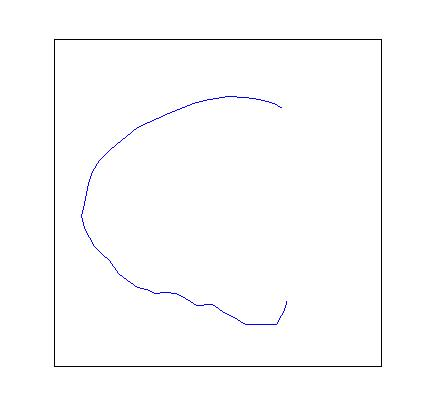
\includegraphics[width=.99\linewidth]{images/cBig}
		\captionof{figure}{C drawn big}
	\end{minipage}%
	\begin{minipage}{.5\textwidth}
		\centering
		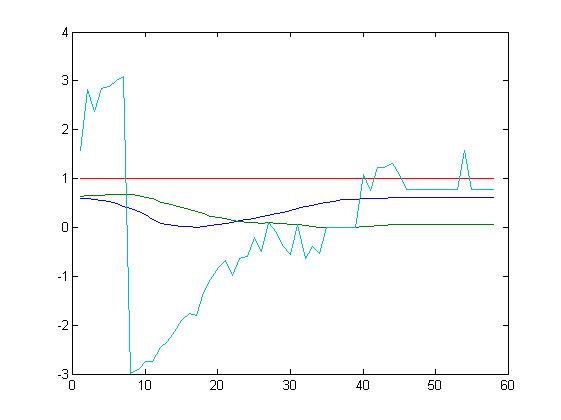
\includegraphics[width=.99\linewidth]{images/cBigPlot}
		\captionof{figure}{Corresponding plot of feature vectors}
	\end{minipage}
\end{figure}
\begin{figure}[H]
	\centering
	\begin{minipage}{.5\textwidth}
		\centering
		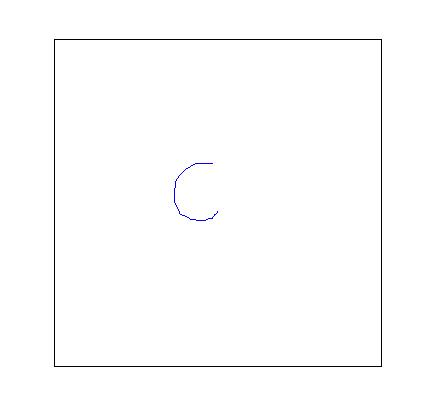
\includegraphics[width=.99\linewidth]{images/cSmall}
		\captionof{figure}{C drawn small}
	\end{minipage}%
	\begin{minipage}{.5\textwidth}
		\centering
		\includegraphics[width=.99\linewidth]{images/cSmallPlot}
		\captionof{figure}{Corresponding plot of feature vectors}
	\end{minipage}
\end{figure}
\begin{figure}[H]
	\centering
	\begin{minipage}{.5\textwidth}
		\centering
		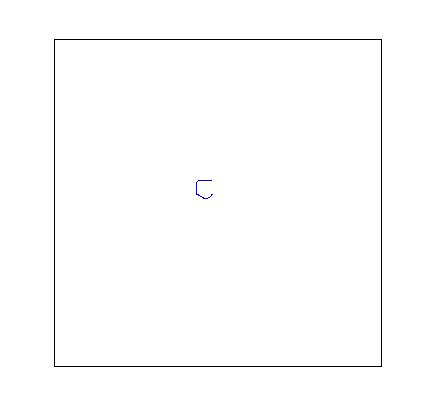
\includegraphics[width=.99\linewidth]{images/cVerySmall}
		\captionof{figure}{C drawn very small}
	\end{minipage}%
	\begin{minipage}{.5\textwidth}
		\centering
		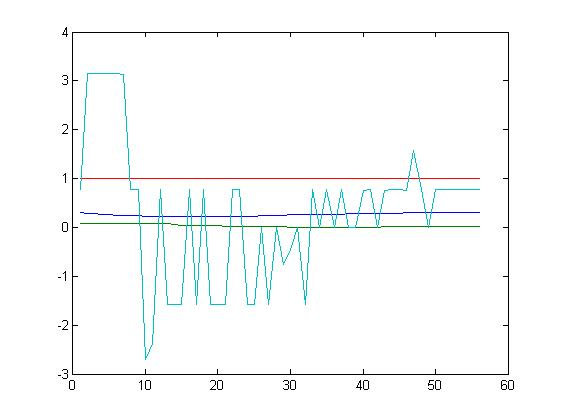
\includegraphics[width=.99\linewidth]{images/cVerySmallPlot}
		\captionof{figure}{Corresponding plot of feature vectors}
	\end{minipage}
\end{figure}

Figure~\ref{fig:o} below shows the plot of the features extracted for the character 'O'. We can observe that though it is mostly similar to the previous plots, it can be seen that there is a difference in the direction vector at the end where it goes beyond the value 1. In the previous plot for character 'C', it can be seen that this direction vector at the end does not mostly go beyond the value 1 . Hence, this attributes to the similarities and differences of the characters 'C' and 'O'.

\begin{figure}[H]
	\centering
	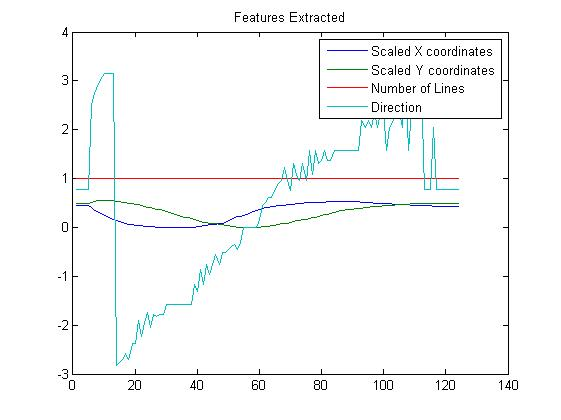
\includegraphics[width=.7\linewidth]{images/deepas/O}
	\caption{Plot of feature vectors for character 'O'}
	\label{fig:o}
\end{figure}

\subsection{Comparison of same character written with different pen movements}
The output feature vectors should not depend on the movements made while the mouse was not pressed, much like a pen that doesn't touch paper shouldn't have an influence on what character is being written.

To test this, we drew the same character ('T') multiple times, while making random mouse movements before drawing the first line, between drawing the lines and after having drawn the second line. The resulting feature vectors are plotted in figure \ref{fig:randT1} and \ref{fig:randT2}.

The difference between these figures is minimal, from which we can conclude that mouse movements while the mouse is not pressed do not affect the resulting feature vectors.

\begin{figure}[H]
	\centering
	\begin{minipage}{.49\textwidth}
		\centering
		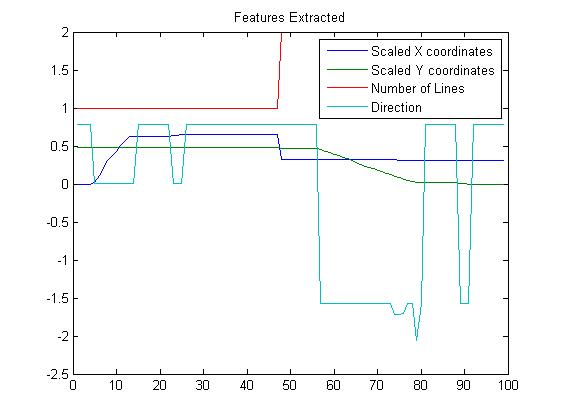
\includegraphics[width=.99\linewidth]{images/deepas/T_random1}
		\captionof{figure}{First drawing of T}
		\label{fig:randT1}
	\end{minipage}
	\begin{minipage}{.49\textwidth}
		\centering
		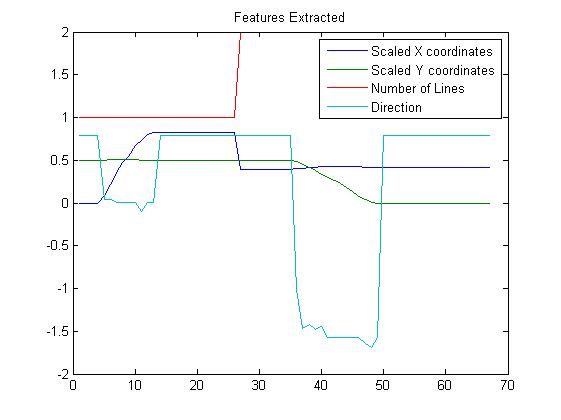
\includegraphics[width=.99\linewidth]{images/deepas/T_random2}
		\captionof{figure}{Another drawing of T}
		\label{fig:randT2}
	\end{minipage}
\end{figure}

\subsection{Differences between 'plus' and 'T'}
The differences between the character 'plus' and 'T' can be seen in the figures below. There is a variation in the magnitude of the value of y coordinates for 'plus' and 'T', as shown in figure~\ref{fig:plus_vs_T_1} and \ref{fig:plus_vs_T_2}

\begin{figure}[H]
	\centering
	\begin{minipage}{.49\textwidth}
		\centering
		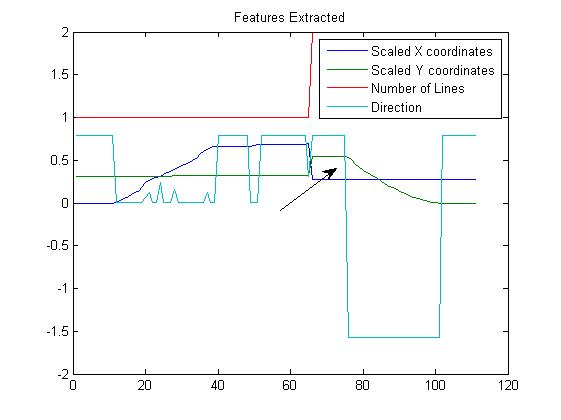
\includegraphics[width=.99\linewidth]{images/deepas/plus}
		\captionof{figure}{Features extracted for '+'}
		\label{fig:plus_vs_T_1}
	\end{minipage}
	\begin{minipage}{.49\textwidth}
		\centering
		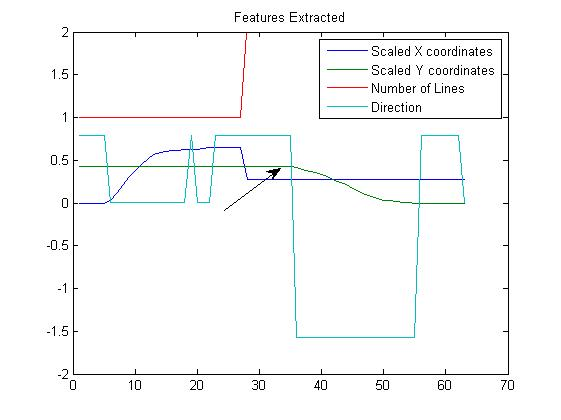
\includegraphics[width=.99\linewidth]{images/deepas/T}
		\captionof{figure}{Features extracted for 'T'}
		\label{fig:plus_vs_T_2}
	\end{minipage}
\end{figure}
 
\subsection{Aspects that are not covered}
The feature extractor that is designed is primarily designed for block letters of English alphabets. This could possibly be extended to cursive handwriting. However, for cursive handwriting recognition, curve fitting could be used to extract curvy features that is predominant in cursive handwriting.  The feature extractor could further be made more robust for random strokes generated between 2 pen movements. The extension could possibly contain some pre-processing where the randomness of the strokes can be filtered out.